\chapter{Evaluation}
\label{c:evaluation}

We integrate our work in GraphflowDB which is an in-memory \gls{gdbms}. It stores the edge and vertex properties as variable-sized records index by their IDs, while adjacency lists are partitioned by edge label-partitioned list of 8-byte vertex and edge IDs. The goal of our experiments is two-fold. First, we show the effectiveness of our columnar storage and compression techniques from the point of memory requirements. We show that redesigning the storage layer of \gls{gdbms} using columns that can harness different types of structures from the graph can compact the storage by up to 4x. Secondly, we evaluate the query performance in light of different optimizations and techniques. In particular, we organize our experiments as follows:

\begin{enumerate}
	\item \textbf{Compression in Adjacency Lists:}  In Section~\ref{exp:adjacency-list-exp} we show the compaction in the size of our adjacency lists by applying the range of optimizations defined Sections~\ref{c:columnar-storage} and~\ref{columnar-compression}. For each of the optimization, we state the cause of the reduction in size and whether it will affect the query performance or not.
	
	\item \textbf{Effectiveness of Single-directional Property Pages:} We compare the performance numbers of order-aware placing of edge properties in the single-directional property pages, as compared to strictly-ordered single-directional property lists as well as unordered edge property columns in Section~\ref{exp:property-pages}.
	
	\item \textbf{Vertex Property Columns for Single Cardinality Edges vs. CSR Adjacency Lists:}  In Section~\ref{exp:single-cardinality} we show the effectiveness of storing single cardinality edges in vertex property columns as compared to vanilla CSR adjacency lists. We compare the performance for both, the uncompressed version and the one compressed by our new prefixSum-based null compression.
	
	\item \textbf{Effectiveness of PrefixSum-based Null Compression:}  Section~\ref{exp:prefixSum} evaluates the overhead in storage and performance by compressing our columns with the new prefixSum-based null compression scheme. It also compares our technique with the vanilla technique mentioned in~\cite{abadi-sparse-col} to show the benefit of using the map instead of iterating over bit-strings.
	
	\item \textbf{List-based Processing vs Volcano-styled Query Execution:} We show the usefulness of list-based processing over the conventional volcano-styled query processing in Section~\ref{exp:list-based}
	
\end{enumerate}

Missing in the experiments is the comparison against the other \gls{gdbms} systems and conventional column stores. We plan to study to the storage and query processing in such systems extensively and also carry out several comparative evaluations, as part of the future work.

\section{Experimental Setup}

\noindent \textbf{Hardware Setup:} For all our experiments, we use a single machine that has two Intel E5-2670 @2.6GHz CPUs and 512 GB of RAM. The machine has 16 physical cores and 32 logical cores. We only use one logical core. We set the maximum size of the JVM heap to 500 GB and keep JVM’s default minimum size.

\begin{figure}
	\hspace{-25pt}
	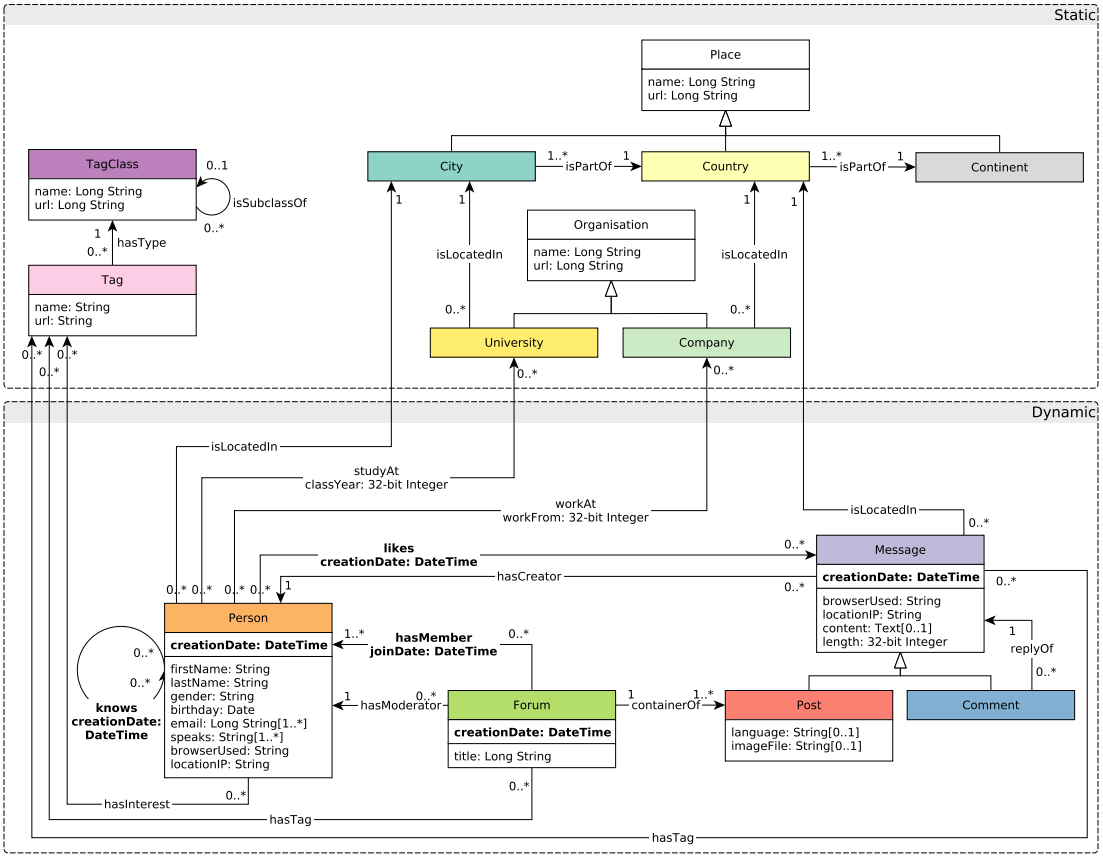
\includegraphics[scale=0.45]{img/ldbc-schema}
	\begin{center}
		\captionsetup{justification=centering}
		\caption{\gls{ldbc} Graph schema. (Obtained from LDBC SNB specification document v0.3.2)}
	\end{center}
	\label{fig:ldbc-schema}
\end{figure}

\noindent \textbf{Datasets:} We use the \gls{ldbc}~\cite{ldbc} dataset generator to generate synthetic graph datasets on which we evaluate all our experiments. \gls{ldbc} is a highly popular, standard tool for benchmarking systems large social graphs. The generated social graph is highly structured which can be seen from the schema in Figure~\ref{ldbc-schema}. Yet, the data is very sparse and have several unstructured edges and properties. Even though the real-world graph varies in the type of structures that exist in them, the \gls{ldbc} data is indicative that most of the graph data are indeed structured.

We generate the data at the scale factor of 100 (\gls{ldbc} 100) that consists of over 1.7 billion edges and 0.3 billion vertices.

\noindent \textbf{Query Workload:} Our query workload mainly consists of short path queries, like k-hop for $k=1,2,3$, with constraint evaluations and aggregations. We base our workloads on the \gls{ldbc} schema. We deliberately concentrate on using short queries as they serve as a stress test for evaluating access from the underlying storage. For instance, a simple 1-hop query tests more rigorously for access from adjacency lists than a query that involves filtering and aggregations. A possible extension could be to evaluate our work using the bigger workloads included in \gls{gdbms}.

\section{Compression in Adjacency Lists}
\label{exp:adjacency-list-exp}

We introduced several optimizations that can make use of the graph data's structure to drastically compact the representation of edges and vertices in the adjacency lists. In this experiment, we demonstrate the memory gains we derive from the incremental application of each optimization on \gls{ldbc} 100. We configure multiple versions of GraphflowDB with a different sets of optimizations and record the size of our forward and backward adjacency lists in each case.

Below are the descriptions of the configurations we use. Each configuration builds on top of previous in the list. 

\begin{enumerate}
	\item \texttt{GF-OLD:} This is our baseline configuration that represents edges and vertices in the adjacency list as 8-byte identifiers. All the adjacency lists are stored in the 2-level CSR structure and are not compressed.
	\item \texttt{+COLS}: Uses vertex property columns from single cardinality edge labels. 
	\item \texttt{+NEW-IDS}: Introduces the new vertex and edge identification scheme, i.e, the vertex ID is represented as a vertex label and an offset. For representing edge, we store a page-level.
	\item \texttt{+0-SUPR}: Implements leading 0 suppression in the components of vertex and edge IDs in adjacency lists.
	\item \texttt{+OMIT}: Omits to store neighbour vertex label and positional offsets of edge IDs wherever possible.
	\item \texttt{+NULL}: Implements prefixSum-based null compression on vertex property columns and adjacency list.
\end{enumerate}

Note that \texttt{+COLS} and \texttt{+NULL} are oblivious to the order in which applied. However, \texttt{+0-SUPR} and \texttt{+OMIT} are not. Since, \texttt{+0-SUPR} is rudimentary in compressing adjacency lists, we order it before \texttt{+OMIT} so that the gains from \texttt{+OMIT} are clear. \texttt{+NEW-IDS} is ordered before \texttt{+0-SUPR} to avoid that benefits of the new edge ID scheme to be overshadowed.

\begin{table}
	\centering
	\begin{tabular}{ |c|c|c|c|c|c|c| } 
		\hline
		& \texttt{GF-OLD} & \texttt{+COLS} & \texttt{+NEW-IDS} & \texttt{+0-CMPRS} & \texttt{+OMIT}& \texttt{+NULL} \\ 
		\hline
		Fwd. Adjacency Lists& 38.25 & 33.25 & 27.22 & 16.35 & 11.14 & 10.53 \\ 
		\hline
		Bwd. Adjacency Lists& 37.93 & 37.50 & 30.93 & 18.75 & 12.79 & 11.15 \\ 
		\hline
		Total& 76.18 & 70.75 & 58.15 & 35.10 & 23.93 & 21.68 \\ 
		\hline \hline
		Bytes per edge& 23.04 & 21.39 & 17.58 & 10.61 & 7.24 & 6.50 \\ 
		\hline
		Reduction Factor& & \textbf{1.08x} & \textbf{1.31x} & \textbf{2.17x} & \textbf{3.18x} & \textbf{3.55x} \\ 
		\hline
	\end{tabular}
	\captionsetup{justification=centering}
	\caption{Memory utilization (in GB) by Adjacency lists of \gls{ldbc} 100. }
	\label{tbl:mem1}
\end{table}

\begin{figure}
	\centering
	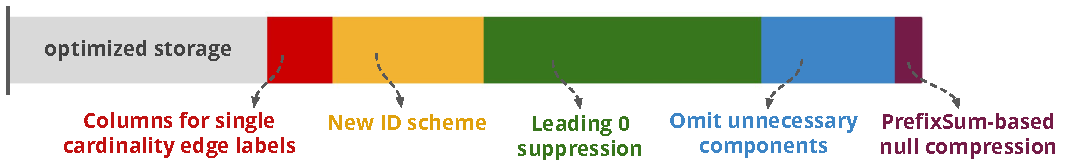
\includegraphics[scale=0.75]{img/opti-breakup}
	\begin{center}
		\captionsetup{justification=centering}
		\caption{Breakup of memory gains by applying different optimizations on Adjacency Lists of \gls{ldbc} scale factor 100 dataset.}
	\end{center}
	\label{fig:opti-breakup}
\end{figure}

Table~\ref{tbl:mem1} shows the memory utiliation (in GB) by the adjacency lists for \gls{ldbc} 100 dataset accross different configurations, while Figure~\ref{fig:opti-breakup} gives the breakup of memory gain per optimization. Gains from \texttt{+COLS} and \texttt{+NULL} are structural and do not change the edge and vertex representation. We evaluate their performance implications in Sections~\ref{exp:single-cardinality} and \ref{exp:prefixSum}. \texttt{+OMIT} greatly benefits from not storing edge's positional offsets since most of the edges do not have properties. Not having to read components 


\section{Effectiveness of Single-Directional Property Pages}
\label{exp:property-pages}

Next, we demonstrate the benefits of reading edge properties from the single-directional property pages.

\section{Vertex Property Columns for Single Cardinality Edges vs. CSR Adjacency Lists}
\label{exp:single-cardinality}

In this experiment, we demonstrate the effectiveness of keeping the edges with the single cardinality label in vertex property columns of either its source or destination vertex. Our goal is two-fold, 1) we show that the storage cost of keeping edges in vertex property columns is significantly less than keeping in 2-level CSR, and 2) accessing edges from vertex property column is more efficient. 

Our workload consist of simple k-hop for $k=1,2,3$. queries on \texttt{replyOf} edges of \gls{ldbc} schema. 

\begin{table}
	\centering
	\begin{subtable}{1\textwidth}
		\centering
		\begin{tabular}{ |c|c|c|c|c| } 
			\hline
			& 1-hop & 2-hop & 3-hop & Memory (in MB) \\ 
			\hline
			2-level CSR Adjacency Lists& 7.03 & 9.13 & 9.60 & 1266.56 \\ 
			\hline
			Vertex Property Columns& 4.34 & 5.80 & 5.85 & 839.93 \\ 
			\hline \hline
			Reduction Factor& \textbf{1.62x} & \textbf{1.57x} & \textbf{1.64x} & \textbf{1.51x} \\ 
			\hline
		\end{tabular}
		\captionsetup{justification=centering}
		\caption{Uncompressed}
		\label{tbl:mem2}
	\end{subtable}
	\begin{subtable}{1\textwidth}
		\centering
		\begin{tabular}{ |c|c|c|c|c| } 
			\hline
			& 1-hop & 2-hop & 3-hop & Memory (in MB) \\ 
			\hline
			2-level CSR Adjacency Lists& 7.78 & 10.40 & 11.23 & 905.23 \\ 
			\hline
			Vertex Property Columns& 5.23 & 8.28 & 8.41 & 478.86 \\ 
			\hline \hline
			Reduction Factor& \textbf{1.49x} & \textbf{1.26x} & \textbf{1.34x} & \textbf{1.89x} \\ 
			\hline
		\end{tabular}
		\captionsetup{justification=centering}
		\caption{Null Compressed}
		\label{tbl:mem2}
	\end{subtable}
	\captionsetup{justification=centering}
	\caption{Vertex property columns vs. 2-level CSR adjacency lists for storing single cardinality edges: Query runtime (in sec) and Memomry usage (in MB)  }
\end{table}

\section{Effectiveness of PrefixSum-based Null compression technique}
\label{exp:prefixSum}

...

\section{List-based Processing vs. Volcano-styles Query Execution}
\label{exp:list-based}

...
